\documentclass[12pt,a4paper]{report}
%\usepackage[utf8]{inputenc}
\usepackage{ulem}
\usepackage{alltt}
\usepackage{amsmath}
\usepackage{amsfonts}
\usepackage{amssymb}
\bibliography{database}
\usepackage{amstext}
\usepackage{listings}
\lstset{
basicstyle=\small\ttfamily,
columns=flexible,
breaklines=true
}
\usepackage{verbatim}
\usepackage{graphicx}
\usepackage{sectsty}
\usepackage{graphicx}
\usepackage[colorlinks]{hyperref}
\usepackage{float}
\addtolength{\oddsidemargin}{-.875in}
\addtolength{\evensidemargin}{-.875in}
\addtolength{\textwidth}{1.75in}
\addtolength{\topmargin}{-.875in}
\addtolength{\textheight}{1.75in}
\usepackage{titlesec}
\titlespacing*{\section}{0pt}{0.5\baselineskip}{\baselineskip}
\setlength{\parindent}{0em}
\setlength{\parskip}{1em}
\author{Oscar Chen, Savith Jayasekera, Charles Chukwukaeme}
\title{WelcomeHomeAB}
\usepackage{graphicx}
\begin{document}
\maketitle
\tableofcontents
\newpage
\section{Abstract}
This report covers the work that was done by the project team in creating a website that caters to customers who are looking to either buy or sell real estate property. The report starts with an introduction of the problem definition and a brief look at the system we are proposing to build to solve this problem. We then move into a discussion of the process of defining the scope of the project. The project definition was accomplished by first putting into plain english what we were trying to accomplish with the system after which we got a first glimpse of what the system would look like with the creation of an Enhanced Entity Relationship Diagram (EERD) and eliciting a list of transactions (and hence functionality) of our system. The implementation section of the report begins with the process we went through to decompose the EERD into a Relational Model. This is followed by a description of Functional Models we used to design the DBMS. Please note that the choice of the framework that we used was made and committed to before we got to the functional model. Therefore the description of the functional model is purely academic as our web application does not depend on SQL statements. We end the report with a documentation of the API we used developed for the project and a user manual of the website. 

\section{Introduction}

Traditions have a way of embedding itself in society's psyche. What was once an innovative idea, perhaps resulting as a function of necessity, becomes so ingrained we stop questioning it and worse accept it as a natural way of life. The process of buying and selling a home has become such a tradition. Most Canadian, if asked, will probably say getting a Realtor is the first step of buying or selling a home. So ingrained is the use of a Realtor in real estate transactions that people don't question the value of the services that they provide anymore.

Realtors serve as brokers of real estate transactions. Given the amounts of money involved they were necessary to serve as guides and middlemen in these transactions. But times have changed and in the technological age most people have become comfortable doing most of their shopping from the comfort of their home. The real advantage of using a realtor nowadays then becomes their access to inventory and the real estate network.

The WelcomeHomeAB project aims to alleviate this problem by connecting home buyers to home sellers. It aims to reduce the costs associated with the process by eliminating commissions from the process. The website will also offer services that is needed in the process of real estate transactions such as: staging, photos, cleaning, inspection, condo document review etc. The motivation behind this project is to make the process of home buying easy and accessible and reduce the associated costs. \par 

We have created a DIY home buying and selling website that will be totally commission free. Users who are looking to sell a property will have the ability to create a profile on the website with which they will be able to add and manage listings of their properties. Users who are looking to buy a property will be able to use our messaging services to connect with home sellers. The website will also host other services like tutorials and step-by-step guides on how to go about buying or selling a property and contact details to a network of contractors and lawyers. An administrator account will be used to control the addition and deletion of these services. The inner workings of the website will be provided in more details in the sections that follow. The landing page of the website is shown in Figure 1.

\begin{figure}[H]
\centering
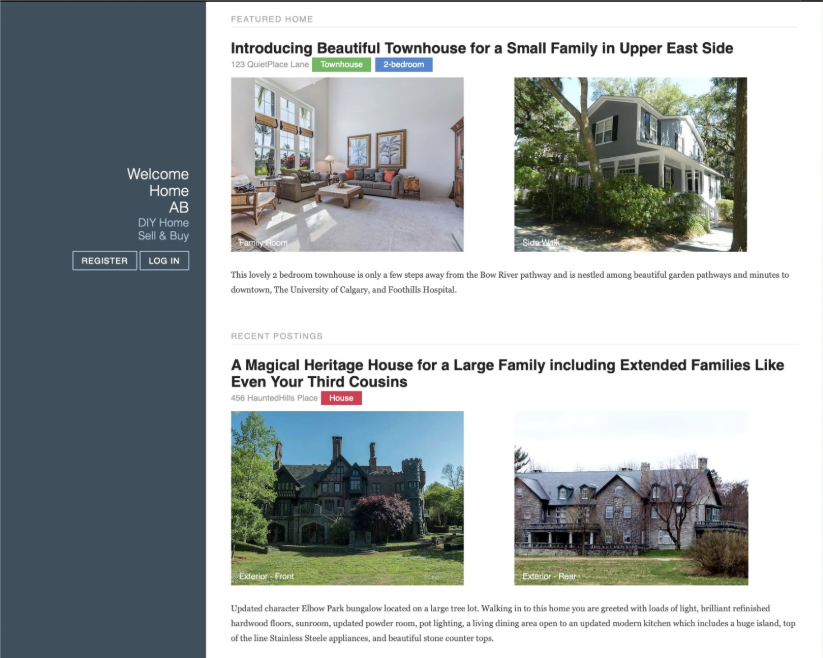
\includegraphics[scale=0.75]{Landingpage.png}
\caption{Website Landing Page}
\label{Figure:landing-page}
\end{figure}   

\section{Project Design} 
This section goes into detail on the design process of the system. We begin with the early stage design process of defining the problem and scope of the project. This is followed by the identification and description of the users of the system. Finally, we provide a preliminary description of the functionality of the system.

\subsection{System Identification}
In order to identify the various components of the system a scope definition was necessary. This was accomplished by providing a description of the system along with the various actors and actions required to run the system. The detailed description of the system is as follows:

\textbf{\textit{WelcomeHomeAB will be designed with the user in mind. Users will be able to list their properties. Users can list multiple properties and any one property will belong to only one user. Users will be required to provide the following for their properties: address, price, lot size, images, and descriptions of the property. Furthermore a user will be able to indicate whether the property is active or not. The system will provide a listing date and a property id. A property can be listed as either commercial or residential. The type of residential property will be indicated (e.g. house, condo, duplex etc). Commercial properties will be identified by the type of businesses they run and the number of units the property has. A property will consist of rooms that can be of different types such as bathrooms, living rooms, garage, kitchen etc. The minimum information required for each room is name, size, description, and an id. Further information for rooms will be required based on the type of room (e.g. a garage will require the number of cars it can hold). The website will also list services that are provided by companies. The type of service that is been provided will be indicated. The companies providing the services will be identified by their name and an id. Both the services listed and the company information will be managed by an administrator. The administrator (admin) will also be able to manage the user accounts. Both users and admins will be required to provide the following information: name, email, phone number(s), user-name and a password. An id will be assigned by the system to both users and admins.}}

The following Enhanced Entity Relationship Diagram (EERD) was produced based on the system description above:

\begin{figure}[H]
\centering
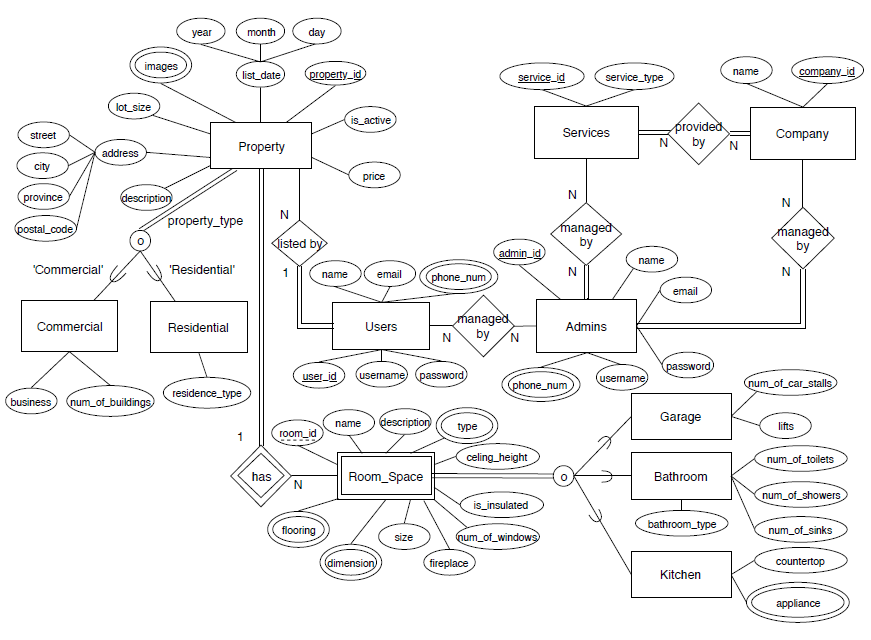
\includegraphics[scale=1.0]{EERD.png}
\caption{Enhanced Entity Relationship Diagram}
\label{Figure:EERD}
\end{figure}   

\subsection{System Users}
The success of our system will depend on the amount of traffic we can get on the website. As a result, it is important that the website be fully accessible to everyone. However, only people who register with the system will be considered a User. The two categories of users are home buyers and home sellers. The information that will be required from a user upon sign-up is as follows:  

\begin{itemize} 
\item Name - First Name (mandatory), Middle Initial(optional), Last Name(mandatory)
\item Phone Number 
\item Username
\item Password
\item Email
\end{itemize}

Once signed up, a User will be able to either view available listings or add one if they have a property to sell. Users of the system will have access to a messaging service with which they can communicate with each other. A User that wants to post a property will be required to provide the following information.

\begin{itemize} 
\item Listing Title
\item Address
\item Price
\item Residence Type
\item Square Footage
\item A full description of the listing
\item Rooms 
\item Images
\end{itemize}

\subsubsection{Service Providers}
The system will be built to be a one-stop shop for real estate transaction. As a result, we will be partnering with companies and organizations that are important in the process of buying or selling a home and listing their services on the website. Some of the service providers that we will be seeking a partnership with include:

\begin{itemize} 
\item Lawyers
\item Financial Institutions 
\item Home inspectors
\item Designers and decorators - for staging homes 
\item Market experts 
\end{itemize}

Companies will not have the ability to make any changes on the website. Instead, all information required to manage their information and the services that they offer will be managed by the system admins. This is to provide some cohesion and vet the information on the services that we offer. In the future, some service providers may be granted more access to the system. 

\subsubsection{System Admins}
The system will have administrators that will manage the day-to-day running of the system. Admins will be able to manage User accounts. They will be solely responsible for managing the companies (and corresponding services) of our partners.

\subsection{Transaction Collection}
In order to elicit a complete picture of the full functionality of our system, a preliminary transaction collection is outlined below.

\begin{itemize} 
\item User sign up, add user authentication to database \par 
This allows a new user (Home-Buyer/Home-Seller) to sign up to the website. This is necessary to unlock the full functionality of the website.

\item User authentication update, email confirmation \par 
This transaction is used to authenticate the information provided by the user. Once authentication is complete, a confirmation email is sent to the user.

\item User profile creation \par 
Once the user information has been authenticated, this transaction creates a profile for the user on the system. 

\item User profile update \par 
This transaction is used to update the profile information of a user. 

\item Property Posting creation \par 
This transaction is responsible for creating an instance of a property in the database by using information entered by a user in the section of the website where users can list properties. 

\item Property Posting update \par 
This transaction is used to update information of an already existing property. This transaction can be activated by a user or a an admin. 

\end{itemize}

This completes the main set of transaction used by our system to carry out instructions provided by the user. The sets of transactions listed below are will be used by a user to either fill out or change the details of a specific property:

\begin{itemize}
\item Property Address creation
\item Property Address update
\item Property Image upload
\item Property Image update
\item Property Room creation
\item Property Room update
\item Custom room type creation
\item Room type update
\end{itemize}

\section{Implementation}
This section of the report describes the processes we went through in order to build the system. It starts with a full description of the decomposition of the EERD into a Relational Model. This is followed by a look at the framework that was used to build the system and how the choice of platform impacted the design of the Database Management System (DBMS). The section concludes with the documentation of the API used and a complete user manual for the website.

\subsection{Relational Model}
The first task of implementation was to transform our EERD into a Relational Model in order to figure out relations and corresponding attributes of our system database. To this end, we applied the 8 steps outlined in the book, Fundamentals of DataBase Syatems\cite{EL}. This process is described in more detail below:

\begin{itemize}
\item \underline{Admin} \par
\textbf{Admin} is a Step 1 decomposition of the strong entity type \textit{Admin} of Figure 2. It's attributes are as follows:
\begin{itemize}
\item admin\_id (Primary Key)
\item username 
\item name
\item email
\item password
\item phone\_num
\end{itemize}
\begin{figure}[H]
\centering
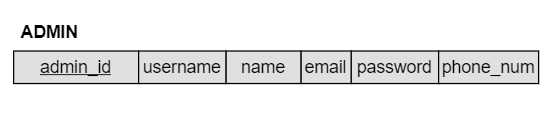
\includegraphics[scale=1.0]{admin.png}
\caption{Relation: Admin}
\label{Figure:admin}
\end{figure}  

\item \underline{User} \par 
\textbf{User} is a Step 1 decomposition of the strong entity type \textit{User} of Figure 2. It's attributes are as follows:
\begin{itemize}
\item user\_id (Primary Key)
\item username 
\item password
\item name
\item email
\end{itemize}
\begin{figure}[H]
\centering
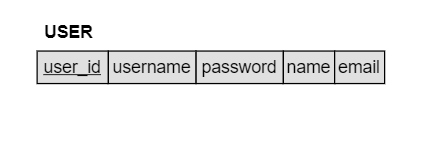
\includegraphics[scale=1.0]{user.png}
\caption{Relation: User}
\label{Figure:user}
\end{figure}  

\item \underline{Property} \par 
\textbf{Property} is a Step 1 decomposition of the strong entity type \textit{Property} of Figure 2 and a Step 8D decomposition of it's sub-classes, Commercial and Residential. It's attributes are as follows:
\begin{itemize}
\item property\_id (Primary Key)
\item user\_id (secondary Key)
\item is\_active
\item price
\item list\_date
\item lot\_size
\item description
\item is\_commercial
\item business
\item num\_of\_buildings
\item is\_residential
\item residence\_type
\end{itemize}
\begin{figure}[H]
\centering
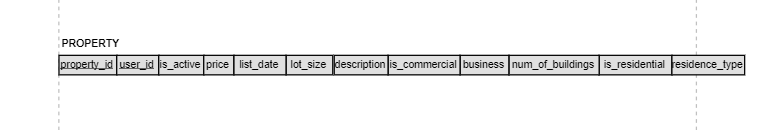
\includegraphics[scale=1.0]{property.png}
\caption{Relation: Property}
\label{Figure:property}
\end{figure} 

\item \underline{Service} \par 
\textbf{Service} is a Step 1 decomposition of the strong entity type \textit{Services} of Figure 2. It's attributes are as follows:
\begin{itemize}
\item service\_id (Primary Key)
\item service\_type
\end{itemize}
\begin{figure}[H]
\centering
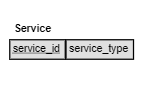
\includegraphics[scale=1.5]{service.png}
\caption{Relation: Service}
\label{Figure:service}
\end{figure}  

\item \underline{Company} \par 
\textbf{Company} is a Step 1 decomposition of the strong entity type \textit{Company} of Figure 2 and the relation \textit{provided by}. It's attributes are as follows:
\begin{itemize}
\item company\_id (Primary Key)
\item service\_id (Secondary Key)
\item name
\end{itemize}
\begin{figure}[H]
\centering
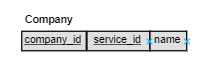
\includegraphics[scale=1.5]{company.png}
\caption{Relation: Company}
\label{Figure:company}
\end{figure}

\item \underline{RoomSpace} \par 
\textbf{RoomSpace} is a Step 2 decomposition of the weak entity type \textit{Room\_Space} of Figure 2. It's attributes are as follows:
\begin{itemize}
\item property\_id (Foreign Key)
\item room\_id (Foreign Key)
\item name
\item description
\item ceiling\_heights
\item is\_insulated
\item num\_of\_windows
\item fireplace
\item size
\end{itemize}
\begin{figure}[H]
\centering
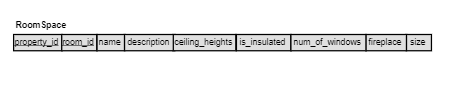
\includegraphics[scale=1.75]{roomspace.png}
\caption{Relation: RoomSpace}
\label{Figure:RS}
\end{figure} 

\item \underline{Service\_managed\_by} \par 
\textbf{Service\_managed\_by} is a Step 5 decomposition of the relationship type \textit{managed by} between the entity types Services and Admins of Figure 2. It's attributes are as follows:

\begin{itemize}
\item service\_id (Foreign Key)  
\item admin\_id (Foreign Key)
\end{itemize}

\begin{figure}[H]
\centering
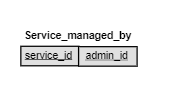
\includegraphics[scale=1.5]{smb.png}
\caption{Relation: Service\_managed\_by}
\label{Figure:smb}
\end{figure} 

\item \underline{Company\_managed\_by} \par 
\textbf{Company\_managed\_by} is a Step 5 decomposition of the relationship type \textit{managed by} between the entity types Company and Admins of Figure 2. It's attributes are as follows:

\begin{itemize}
\item company\_id (Foreign Key)  
\item admin\_id (Foreign Key)
\end{itemize}

\begin{figure}[H]
\centering
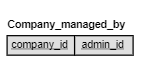
\includegraphics[scale=1.5]{cmb.png}
\caption{Relation: Company\_managed\_by}
\label{Figure:cmb}
\end{figure} 

\item \underline{PropertyAddress} \par 
\textbf{PropertyAddress} is a decomposition of the composite attribute \textit{address} of the entity type \textit{Property} of Figure 2. Note that the decomposition of a composite attribute is not part of the 8 steps outlined in \cite{EL}. This decomposition was done because we believe that address is an important enough information to store in the database that a separate table for it is a good idea.

\begin{figure}[H]
\centering
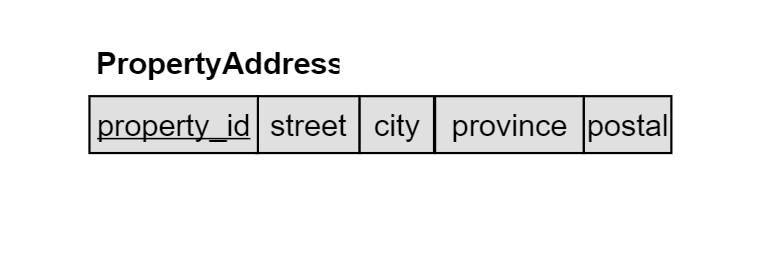
\includegraphics[scale=0.5]{PA.png}
\caption{Relation: PropertyAddress}
\label{Figure:pa}
\end{figure} 

\item \underline{User\_managed\_by} \par 
\textbf{User\_managed\_by} is a Step 5 decomposition of the relationship type \textit{managed by} between the entity types \textit{User} and \textit{Admins} of Figure 2. It's attributes are as follows:

\begin{itemize}
\item user\_id (Foreign Key)  
\item admin\_id (Foreign Key)
\end{itemize}

\begin{figure}[H]
\centering
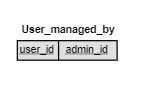
\includegraphics[scale=1.5]{umb.png}
\caption{Relation: User\_managed\_by}
\label{Figure:umb}
\end{figure}

\item \underline{PhoneNumber} \par 
\textbf{PhoneNumber} is a Step 6 decomposition of the multivalued attribute \textit{phone\_num} of the entity type \textit{User} of Figure 2. It's attributes are as follows:

\begin{itemize}
\item user\_id (Foreign Key)  
\item phone\_num 
\end{itemize}

\begin{figure}[H]
\centering
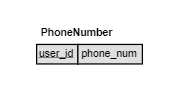
\includegraphics[scale=1.5]{phone.png}
\caption{Relation: PhoneNumber}
\label{Figure:phone}
\end{figure}

\item \underline{PropertyImages} \par 
\textbf{PropertyImages} is a Step 6 decomposition of the multivalued attribute \textit{images} of the entity type \textit{Property} of Figure 2. It's attributes are as follows:

\begin{itemize}
\item property\_id (Foreign Key)  
\item image 
\end{itemize}

\begin{figure}[H]
\centering
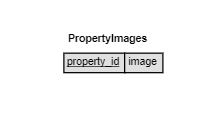
\includegraphics[scale=1.5]{img.png}
\caption{Relation: PropertyImages}
\label{Figure:img}
\end{figure}

\item \underline{RoomDimension} \par 
\textbf{RoomDimension} is a Step 6 decomposition of the multivalued attribute \textit{dimension} of the entity type \textit{Room\_Space} of Figure 2. It's attributes are as follows:

\begin{itemize}
\item property\_id (Foreign Key)  
\item room\_id (Foreign Key)
\item dimension 
\end{itemize}

\begin{figure}[H]
\centering
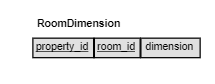
\includegraphics[scale=1.5]{rmdim.png}
\caption{Relation: RoomDimension}
\label{Figure:rmdim}
\end{figure}

\item \underline{RoomFlooring} \par 
\textbf{RoomFlooring} is a Step 6 decomposition of the multivalued attribute \textit{flooring} of the entity type \textit{Room\_Space} of Figure 2. It's attributes are as follows:

\begin{itemize}
\item property\_id (Foreign Key)  
\item room\_id (Foreign Key)
\item flooring
\end{itemize}

\begin{figure}[H]
\centering
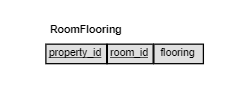
\includegraphics[scale=1.5]{rmflr.png}
\caption{Relation: RoomFlooring}
\label{Figure:rmflr}
\end{figure}

\item \underline{RoomKitchen} \par 
\textbf{RoomKitchen} is a Step 8A decomposition of the subclass \textit{Kitchen} of the entity type \textit{Room\_Space} of Figure 2. It's attributes are as follows:

\begin{itemize}
\item property\_id (Foreign Key)  
\item room\_id (Primary Key)
\item countertop
\end{itemize}

\begin{figure}[H]
\centering
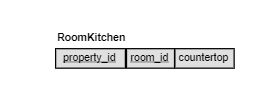
\includegraphics[scale=1.5]{rmktch.png}
\caption{Relation: RoomKitchen}
\label{Figure:rmktch}
\end{figure}

\item \underline{KitchenAppliance} \par 
\textbf{KitchenAppliance} is a Step 6 decomposition of the multivalued attribute \textit{appliance} of the entity type \textit{Kitchen} of Figure 2. It's attributes are as follows:

\begin{itemize}
\item property\_id (Foreign Key)  
\item room\_id (Foreign Key)
\item appliance
\end{itemize}

\begin{figure}[H]
\centering
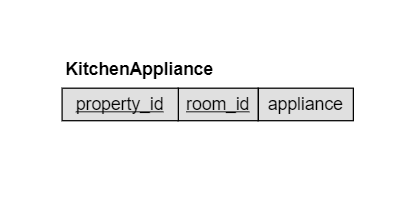
\includegraphics[scale=1.0]{ktchapp.png}
\caption{Relation: KitchenAppliance}
\label{Figure:ktchapp}
\end{figure}

\item \underline{RoomBathroom} \par 
\textbf{RoomBathroom} is a Step 8A decomposition of the subclass \textit{Bathroom} of the entity type \textit{Room\_Space} of Figure 2. It's attributes are as follows:

\begin{itemize}
\item property\_id (Foreign Key)  
\item room\_id (Primary Key)
\item num\_of\_toilets 
\item num\_of\_showers 
\item num\_of\_sinks 
\item bathroom\_type 
\end{itemize}

\begin{figure}[H]
\centering
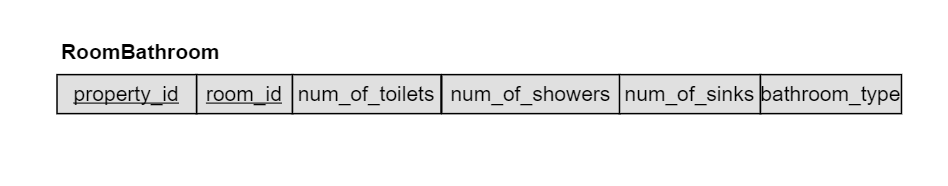
\includegraphics[scale=1.0]{rmbthrm.png}
\caption{Relation: RoomBathroom}
\label{Figure:rmbthrm}
\end{figure}

\item \underline{RoomGarage} \par 
\textbf{RoomGarage} is a Step 8A decomposition of the subclass \textit{Garage} of the entity type \textit{Room\_Space} of Figure 2. It's attributes are as follows:

\begin{itemize}
\item property\_id (Foreign Key)  
\item room\_id (Primary Key)
\item num\_of\_car\_stalls
\item lifts
\end{itemize}

\begin{figure}[H]
\centering
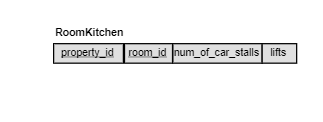
\includegraphics[scale=1.5]{rmgrg.png}
\caption{Relation: RoomGarage}
\label{Figure:rmgrg}
\end{figure}

\end{itemize}

The full relational model is shown in Figure 9 along with constraints between relations. These relations form the schemas of that the design of our DBMS is based on.
\begin{figure}[H]
\centering
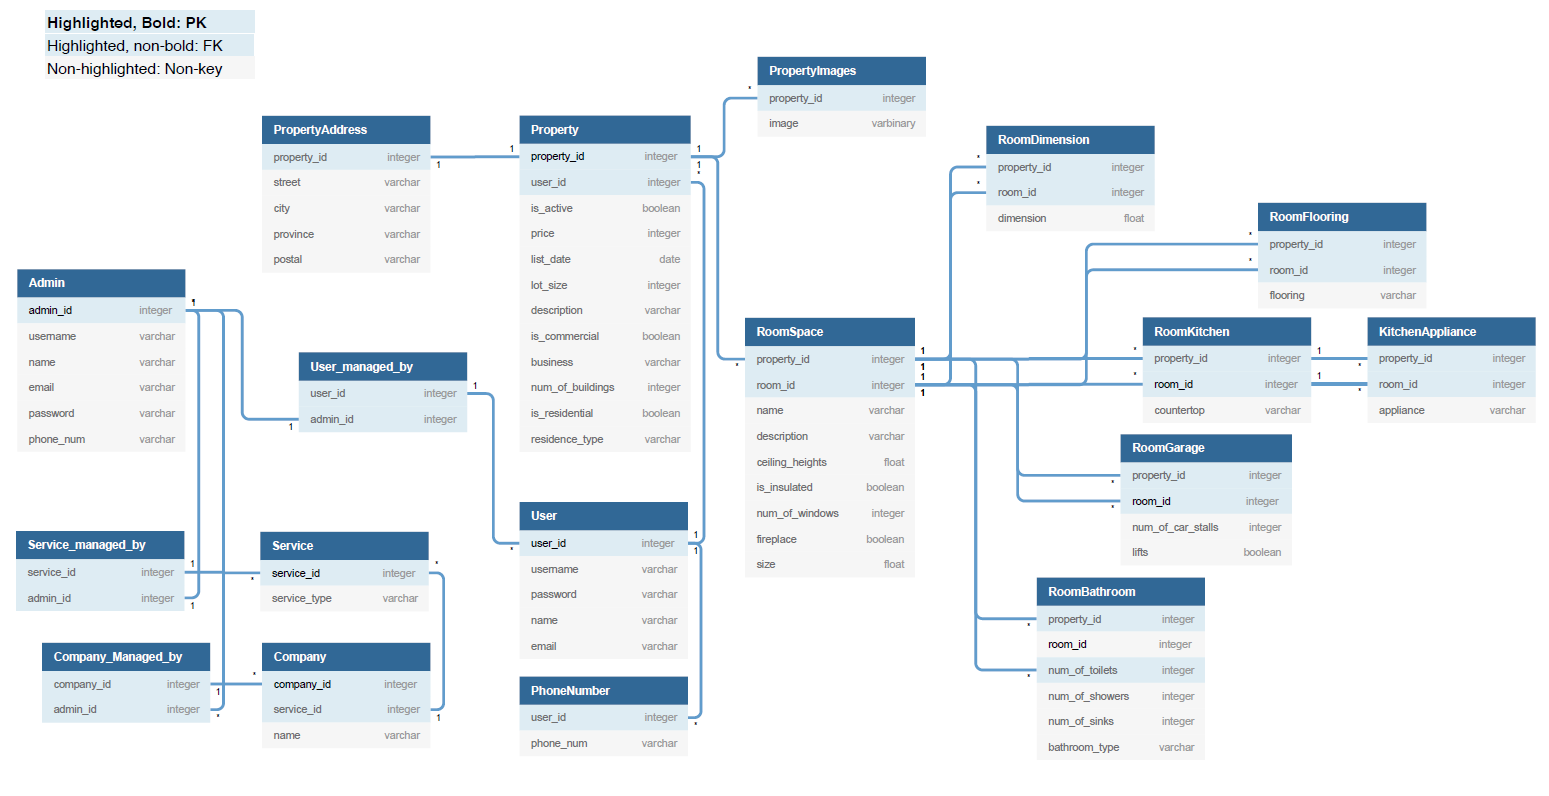
\includegraphics[scale=0.5]{RelationalModel.png}
\caption{Relational Model}
\label{Figure:RM}
\end{figure} 

\subsection{DBMS Design}
Before we discuss our design we will go into a brief summary of the Django framework which is what we used for the design of our system. Understanding this framework will make it easier to understand the design choices we made as we transitioned the Relational Model into an actual database. \par 

Django, which is an open-source web development framework, is based on the Python language\cite{DJ}. The important thing to understand about the Django framework, for the purpose of this report, is that it is based on a Model-View-Template architectural pattern as shown in the figure below:
\begin{figure}[H]
\centering
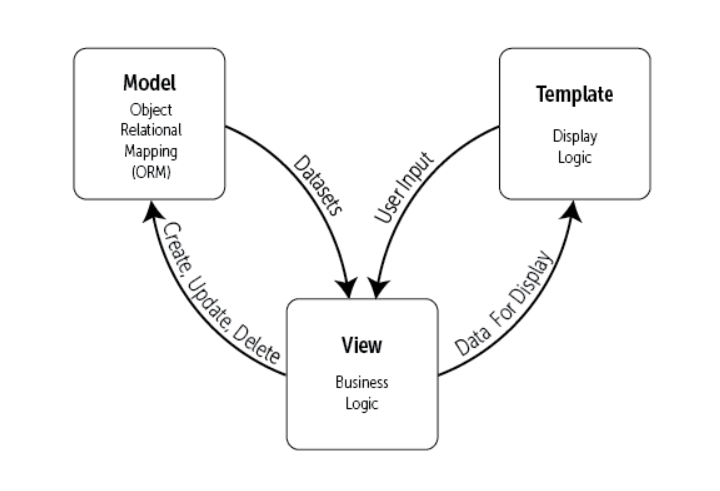
\includegraphics[scale=1.0]{MVT.png}
\caption{Django's M-V-T Architecture Pattern \cite{DJ2}}
\label{Figure:MVT}
\end{figure} 

This structure is a variation on the MVC design model that is widely used in the industry so we won't go into it in detail here. The key things to know for this section all revolves around the Model and they are as follows:

\begin{itemize}

\item \textbf{\underline{Django Models}} \par
Django uses a python class for managing the information that a system uses \cite{dj}. 
These classes are called models and they contain the fields/attributes and behaviors of the data that we are working with. In essence, a model refers to single relation in the database. For example the relations Property and User will have 2 different models in the Django. 

\textbf{\underline{Django Ojects}} \par 
An object refers to instance of the model classes. For example the Property model will have objects that refer to different instances of a property. An object is basically a tuple in the relational model. \cite{DJ2} 

\textbf{\underline{Django ORM}} \par
Django manages the interaction between the system and the underlying database using Object-Relational Mapping (ORM). When a model is created in Django, a corresponding table is automatically created in the database. This is the function of the ORM. It provides an easy way to transfer (or map) data between the models and the underlying database. What this means is that databases that are connected to a Django application \textbf{do not use SQL statements} to manipulate the data stored in the database. \par 

\end{itemize}

What this means for our system is that we do not actually need SQL statements for our system. Nonetheless, for the completeness of this report and in case we decide to implement this system using a different framework, we outline the SQL statements that we generated during the design phase of this project.  \par 

We implemented our DBMS using MySQL. The relational model of our system formed the basis of the design of our database. The relations that was identified during decomposition of the EERD model formed the first revisions of the relations that we would be creating in a database schema but in order to identify the interactions and structure of the database we produced two functional model: Hierarchy Input Process Output Diagram (HIPO) and a Data Flow Diagram (DFD).

\begin{itemize}
\item \textbf{\underline{Hierarchy Input Process Output Diagram}} \par 
HIPO is used to graphically represent the control structure of a system. It is a chart that is based on a hierarchy of the system and describes the functions performed by each module of the system \cite{CL}. We created our HIPO diagram using a careful consideration of our EERD (Figure 2) and the transaction collections identified from the project design. The HIPO diagram for our system is shown in the figure below:

\begin{figure}[H]
\centering
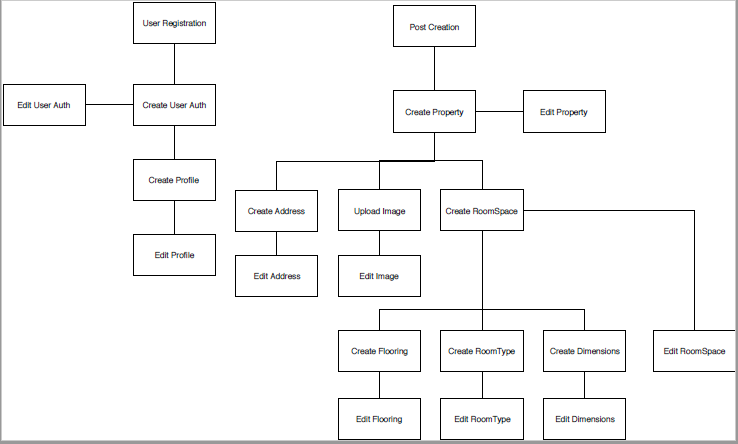
\includegraphics[scale=1.0]{hipo.png}
\caption{Hierarchy Input Process Output Diagram (HIPO)}
\label{Figure:hipo}
\end{figure}

From the HIPO diagram we can see that there are two basic functionality of our system: the creation and management of user profiles and the creation and management of properties in the system. Note that management refers to add, edit and delete operations.

\item \textbf{\underline{Data Flow Diagram}} \par 
The Data Flow Diagram (DFD) provides another functional perspective of the system. A DFD can provides us with a picture of the movement of data within the system \cite{CL}. Data movement in a DFD is described in relation to the external entities of the system and the processes and data stores within the system. An entity is any external actor that interact with the system (e.g. users, admins, services etc). A process is any function within the system that transforms data. We provided two levels of the DFD of our system as shown in the figures below.

\begin{figure}[H]
\centering
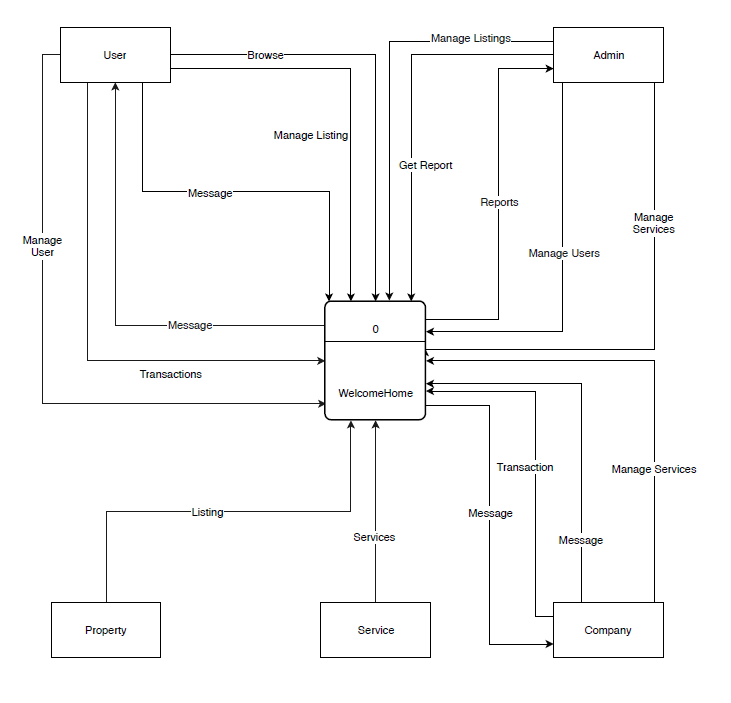
\includegraphics[scale=1.0]{dfd1.png}
\caption{Level 1 DFD (Context Diagram)}
\label{Figure:dfd1}
\end{figure}

\begin{figure}[H]
\centering
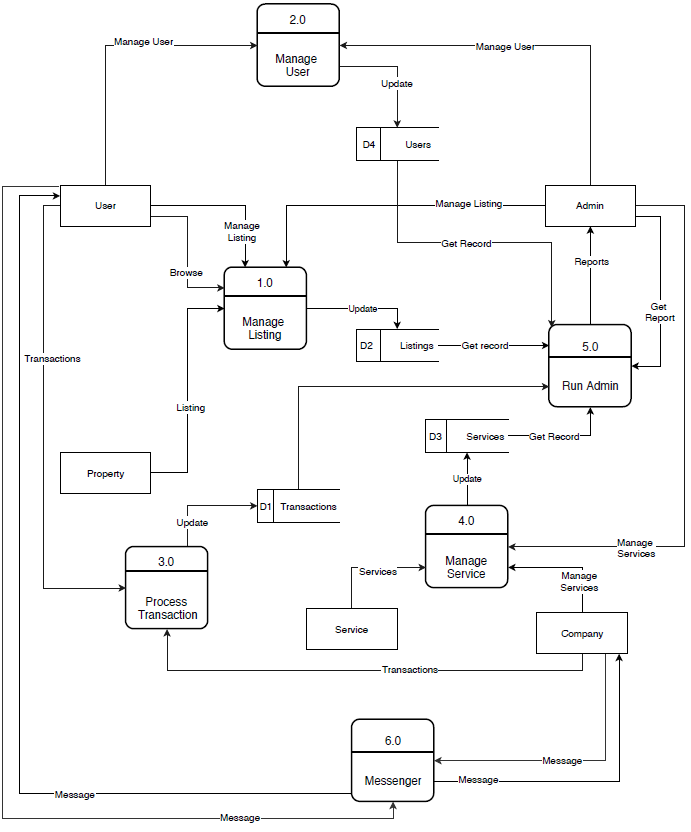
\includegraphics[scale=1.0]{dfd2.png}
\caption{Level 2 DFD}
\label{Figure:dfd2}
\end{figure}

The level 1 of the DFD, also known as the Context Diagram, in addition to the functionality shown in the HIPO includes more processes that we would like from the system such as transactions and administrative services (bookkeeping). Level 2 just goes into more details on these topics.
\end{itemize}

With these diagrams in mind we constructed the SQL statements that can be used to manage our database. The construction of these diagrams were insightful as it allowed us to identify some functionality that we had not considered during the project design phase such as transaction and bookkeeping. But we will not be fully implementing all of these in the report and web application as they fall outside the scope we had defined for the project.  

\subsubsection{SQL Statements}
We wrote SQL statements to define the two broad category of function identified from our functional model. The statements are listed below:

\begin{itemize}
\item Creation and Management of User Profiles
\begin{center}
\begin{lstlisting}
-- User sign up, add user authentication to database
INSERT INTO welcomehome.auth_user (id, password, last_login, is_superuser, username, first_name, last_name, email, is_staff, is_active, date_joined) VALUES (1, 'pbkdf2_sha256$120000$BfmJVD105WeJ$4/8aES7lC4mld/KJQTz4afF7hZWF2LwobueDL6HpgoA=', '', 0, 'usernameX', '', '', '', 0, 0, '2019-03-16 00:40:02.905475');

-- User authentication update, email confirmation
UPDATE welcomehome.auth_user SET password = 'pbkdf2_sha256$120000$BfmJVD105WeJ$4/8aES7lC4mld/KJQTz4afF7hZWF2LwobueDL6HpgoA=', last_login = '2019-03-16 04:03:02.442649', is_superuser = 0, username = 'usernameX', first_name = '', last_name = '', email = '', is_staff = 0, is_active = 1, date_joined = '2019-03-16 00:40:02.905475' WHERE id = 1;

-- User profile creation
INSERT INTO welcomehome.global_listing_userprofile (id, email, phone_day, phone_alt, user_id) VALUES (1, 'oscar@chen.com', '40312345678', null, 1);

-- User profile update
UPDATE welcomehome.global_listing_userprofile SET email = 'oscar@chen.com', phone_day = '40312345678', phone_alt = null, user_id = 1 WHERE id = 1;

\end{lstlisting}
\end{center}

\item Creation and Management of Properties
\begin{center}
\begin{lstlisting}
-- Property Posting creation
INSERT INTO welcomehome.global_listing_property (property_id, is_active, price, list_date, above_grade_sqft, lot_size, post_title, post_priority, description, is_commercial, business, num_of_buildings, is_residential, residence_type, user_id) VALUES (1, 1, 1000000, '2019-03-10', 1500, 2000, 'Introducing Beautiful Townhouse for a Small Family in Upper East Side', 0, 'This lovely 2 bedroom townhouse is only a few steps away from the Bow River pathway and is nestled among beautiful garden pathways and minutes to downtown, The University of Calgary, and Foothills Hospital.', 0, '', 1, 1, 'Townhouse', 1);

-- Property Posting update
UPDATE welcomehome.global_listing_property SET is_active = 1, price = 1000000, list_date = '2019-03-10', above_grade_sqft = 1500, lot_size = 2000, post_title = 'Introducing Beautiful Townhouse for a Small Family in Upper East Side', post_priority = 0, description = 'This lovely 2 bedroom townhouse is only a few steps away from the Bow River pathway and is nestled among beautiful garden pathways and minutes to downtown, The University of Calgary, and Foothills Hospital.', is_commercial = 0, business = '', num_of_buildings = 1, is_residential = 1, residence_type = 'Townhouse', user_id = 1 WHERE property_id = 1;

-- Property Address creation
INSERT INTO welcomehome.global_listing_propertyaddress (id, street, city, province, postal, property_id_id) VALUES (1, '123 Happy Lane', 'Calgary', 'AB', 'T3R2D4', 1);

-- Property Address update
UPDATE welcomehome.global_listing_propertyaddress SET street = '123 Happy Lane', city = 'Calgary', province = 'AB', postal = 'T3R2D4', property_id_id = 1 WHERE id = 1;

-- Property Image upload
INSERT INTO welcomehome.global_listing_propertyimages (id, image, title, property_id_id) VALUES (1, 'temp/1A.jpg', 'im1', 1);

-- Property Image update
UPDATE welcomehome.global_listing_propertyimages SET title = 'im1', image = 'temp/1A.jpg', property_id_id = 1 WHERE id = 1;

-- Property Room creation
INSERT INTO welcomehome.global_listing_roomspace (id, room_id, name, description, ceiling_heights, is_insulated, num_of_windows, fireplace, size, property_id_id) VALUES (1, 1, 'Kitchen', 'A place to cook', 12, 1, 2, 0, 400, 1);

-- Property Room update
UPDATE welcomehome.global_listing_roomspace SET room_id = 1, name = 'Kitchen', description = 'Kitchen', ceiling_heights = 12, is_insulated = 1, num_of_windows = 2, fireplace = 0, size = 400, property_id_id = 1 WHERE id = 1;

-- Custom room type creation
INSERT INTO welcomehome.global_listing_roomtype (id, room_type, property_id_id, room_id_id) VALUES (1, 'Kitchen2', 1, 2);

-- Room type update
UPDATE welcomehome.global_listing_roomtype SET room_type = 'Kitchen', property_id_id = 1, room_id_id = 1 WHERE id = 1;

-- Room flooring creation
INSERT INTO welcomehome.global_listing_roomflooring (id, flooring, property_id_id, room_id_id) VALUES (1, 'Hard wood', 1, 1);

-- Room flooring update
UPDATE welcomehome.global_listing_roomflooring SET flooring = 'Hard wood', property_id_id = 1, room_id_id = 1 WHERE id = 1;

-- Room dimensions creation
INSERT INTO welcomehome.global_listing_roomdimension (id, dimension, property_id_id, room_id_id) VALUES (1, 20, 1, 1);
INSERT INTO welcomehome.global_listing_roomdimension (id, dimension, property_id_id, room_id_id) VALUES (2, 15, 1, 1);

-- Room dimension update
UPDATE welcomehome.global_listing_roomdimension SET dimension = 20, property_id_id = 1, room_id_id = 1 WHERE id = 1;
UPDATE welcomehome.global_listing_roomdimension SET dimension = 15, property_id_id = 1, room_id_id = 1 WHERE id = 2;
\end{lstlisting}
\end{center}
\end{itemize}

\section{API Documentation}
Information within our database can be accessed using our RestfulAPI. The allowed request types are: 
\begin{itemize}
\item GET
\item HEAD
\item OPTIONS
\end{itemize}

The current version of the API can be accessed by links provided in the following endpoint: \verb|/api-info| \par 

There are two main data types that can be accessed from the API: 
\begin{itemize}
\item Properties
\item \verb|Company & Services|
\end{itemize}

The following endpoints provide direct access to an array containing all instances of the above types in the JSON format.

\begin{itemize}
\item Property: \verb|/global_listing/api/property/?format=json|
\item Services: \verb|/services/api/company/?format=json|
\end{itemize}

\newpage
\section{User Manual}


\newpage
\begin{appendix}
  \listoffigures
\end{appendix}


\begin{thebibliography}{10}
\bibitem{EL} R. Elmasri and S. B. Navathe, Fundamentals of database systems. Harlow, Essex: Pearson Education, 2017.
\bibitem{DJ} URL https://docs.djangoproject.com/en/2.2/topics/db/models/
Website Title Django
Article Title Documentation
Date Accessed April 16, 2019
\bibitem{DJ2} URL https://djangobook.com/django-tutorials/django-overview/
Website Title The Django Book
Article Title Django Overview
Date Published December 24, 2017
Date Accessed April 16, 2019
\bibitem{CL} ENSF 619 L06 - Lecture/Tutorial Notes
\end{thebibliography}
\end{document}
